\documentclass[../main.tex]{subfiles}
\usepackage{graphicx}
%~2200 Worte
\begin{document}
\subsection{Systemarchitektur} %Tim
\subsubsection{Architekturmuster}
\subsubsection{Entscheidungsfindung \& spezifische Auswahl}

\subsection{Datenbankdesign} %Tim
\subsubsection{Datenmodell}
\subsubsection{Datenbanksystemauswahl}

\subsection{Backend-Design} %Tim
\subsubsection{Notwendige API-Abfragen}
\subsubsection{Backend-Framework Entscheidung}

\subsection{GUI-Design \& Frontend-Frameworks} %Lauritz
\subsubsection{Gestaltungsprozess}
Der Designprozess der grafischen Benutzeroberfläche (GUI) begann mit der Erstellung einfacher Diagramme auf 
draw.io (siehe Bild). Diese initiale Skizzierung fokussierte sich zunächst auf die Startseite, welche die Karte und den Live 
Feed umfasste, und wurde später um die Eingabeseite für das Eintragen eines Pilzes erweitert. Diese konzeptionelle Phase 
erfolgte in einer gemeinsamen Brainstorming-Session, in der Ideen frei ausgetauscht und Entwürfe entwickelt und verglichen 
wurden.

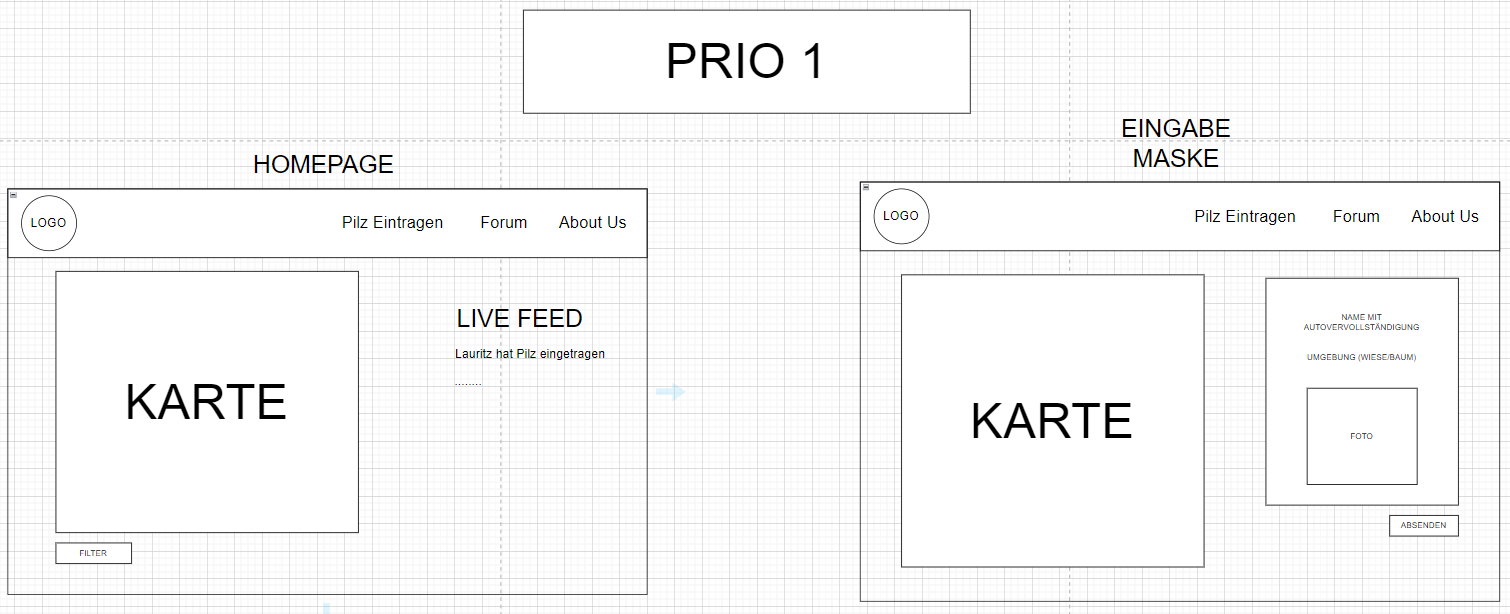
\includegraphics{..\\abbildungen\\GUI_Entwurf_Drawio.jpg}

Nicht-funktionale Anforderungen wie Einfachheit, Benutzerfreundlichkeit und Responsive Design waren hierbei maßgebliche 
Faktoren, an denen sich der Designprozess orientierte. Die Einfachheit der Benutzeroberfläche wurde als essenziell erachtet, 
um die Nutzerführung intuitiv und zugänglich zu gestalten. So wurde jedes Element der GUI, sowie deren Anordnung, mit dem Ziel 
entworfen, eine direkte und unkomplizierte Interaktion möglich zu machen. Benutzerfreundlichkeit stand ebenfalls im Vordergrund, 
um sicherzustellen, dass Nutzer aller Erfahrungsstufen die Anwendung problemlos verwenden können. So gibt es keine überflüssigen
Elemente und die vorhandenen sind gut sichtbar und selbsterklärend. Die Anpassung an verschiedene Endgeräte durch ein Responsive 
Design war ein weiterer kritischer Aspekt, der ebenfalls Berücksichtigung fand. Da die Applikation höhst wahrscheinlich schon 
während des Pilzesuchens verwendet wird, gewährleistet das Responsive Design, dass "ShroomScout" auf Smartphones gleichermaßen 
funktionell und ästhetisch ansprechend ist, wie auf Desktops und Tablets.

\subsubsection{Frontend-Framework Entscheidung}
Nach der Gestaltung der GUI stand letztlich noch die Auswahl eines Frontend-Frameworks an. Ein Frontend-Framework ist eine Sammlung 
wiederverwendbarer Designvorlagen und Code-Snippets, die Entwicklern helfen, konsistente und effiziente Benutzeroberflächen 
zu erstellen. Diese Frameworks bieten vorgefertigte Komponenten und Werkzeuge, die die Entwicklung beschleunigen und die 
Einhaltung von Webstandards erleichtern.

Die Entscheidung fiel recht schnell auf Angular, hauptsächlich aufgrund von bereits vorhandenen Erfahrungen und aufgebautem
Basiswissen mit der Technologie. Obwohl andere Frontend-Frameworks wie React und Vue ebenfalls in Betracht gezogen wurden, 
gab die Vertrautheit mit Angular den Ausschlag. React, bekannt für seine Flexibilität und Leistung, und Vue, geschätzt für 
seine Einfachheit und leichtes Lernen, sind ebenfalls hervorragende Optionen für die Entwicklung moderner Webanwendungen. Die 
Entscheidung für Angular basierte jedoch auf der spezifischen Projekterfahrung und dem Komfortniveau der Entwickler. 

Darüber hinaus lassen sich weitere Vorteile von Angular, bzw. generell eines Frontend-Frameworks finden, welche den Entwicklungsprozess
des Frontends unterstützten:

\begin{itemize}

  \item 
  Angular überzeugt durch eine komponentenbasierte Architektur und dadurch modulare Herangehensweise bei der Entwicklung.
  Jeder Baustein der Anwendung wird dabei in einer Komponente gekapselt, was Klarheit der Anwendungsstruktur fördert und die Wiederverwendung
  dieser Komponenten möglich macht.

  \item 
  Die Bereitstellung umfangreicher Bibliotheken von eingebauten Funktionen und Diensten, wie Formularverwaltung, Routing oder ein HTTP-Client, 
  bietet signifikante Vorteile.

  \item 
  Die Verwendung von TypeScript, welches JavaScript um starke Typisierung und objektorientierte Programmierkonzepte wie Klassen, Interfaces und 
  Dekoratoren erweitert, ermöglicht eine deutlich verbesserte Entwicklungserfahrung.
  
  \item 
  Angular ermöglicht durch seine umfangreiche Dokumentation und Community-Unterstützung eine effiziente Problemlösung und Weiterentwicklung.
  
\end{itemize}

\end{document}
